\section{GPUE: GPU Gross--Pitaevskii equation solver}\label{sec:GPUE}

Given the effectiveness of GPU computing in the simulation of the linear Sch\"odinger equation system for SAP, we next applied the newly-developed techniques to simulating Bose--Einstein condensates, which formed the bulk of work during my thesis. The body of software developed for this project has been released as the tool ``GPUE'', available at \url{https://github.com/mlxd/gpue}~\cite{MLXD_GPUE}. Performance testing of this code was carried out by Peter Wittek, ICFO, Barcelona~\cite{Wittek:2016}. A comparison was performed between GPUE, the Trotter--Suzuki (TS) package developed by Wittek \textit{et} al. \cite{NUM:Wittek_cpc_2013}, and the mature GPELab software suite for MATLAB \cite{NUM:GPElab_1,NUM:GPElab_2}. The sample results taken for time evolution are given in Fig.~\ref{fig:gpuevsts}. GPUE and GPU-enabled TS clearly beat MATLAB, and CPU performance by a significant margin. Although TS is a more generalised suite for computing, as far as we are currently aware the GPU computation does not yet allow for Gross--Pitaevskii solutions with angular momentum. GPUE is currently the optimal choice for rotating condensate systems out of the examined software suites.

\begin{figure}[htb]
    \centering
    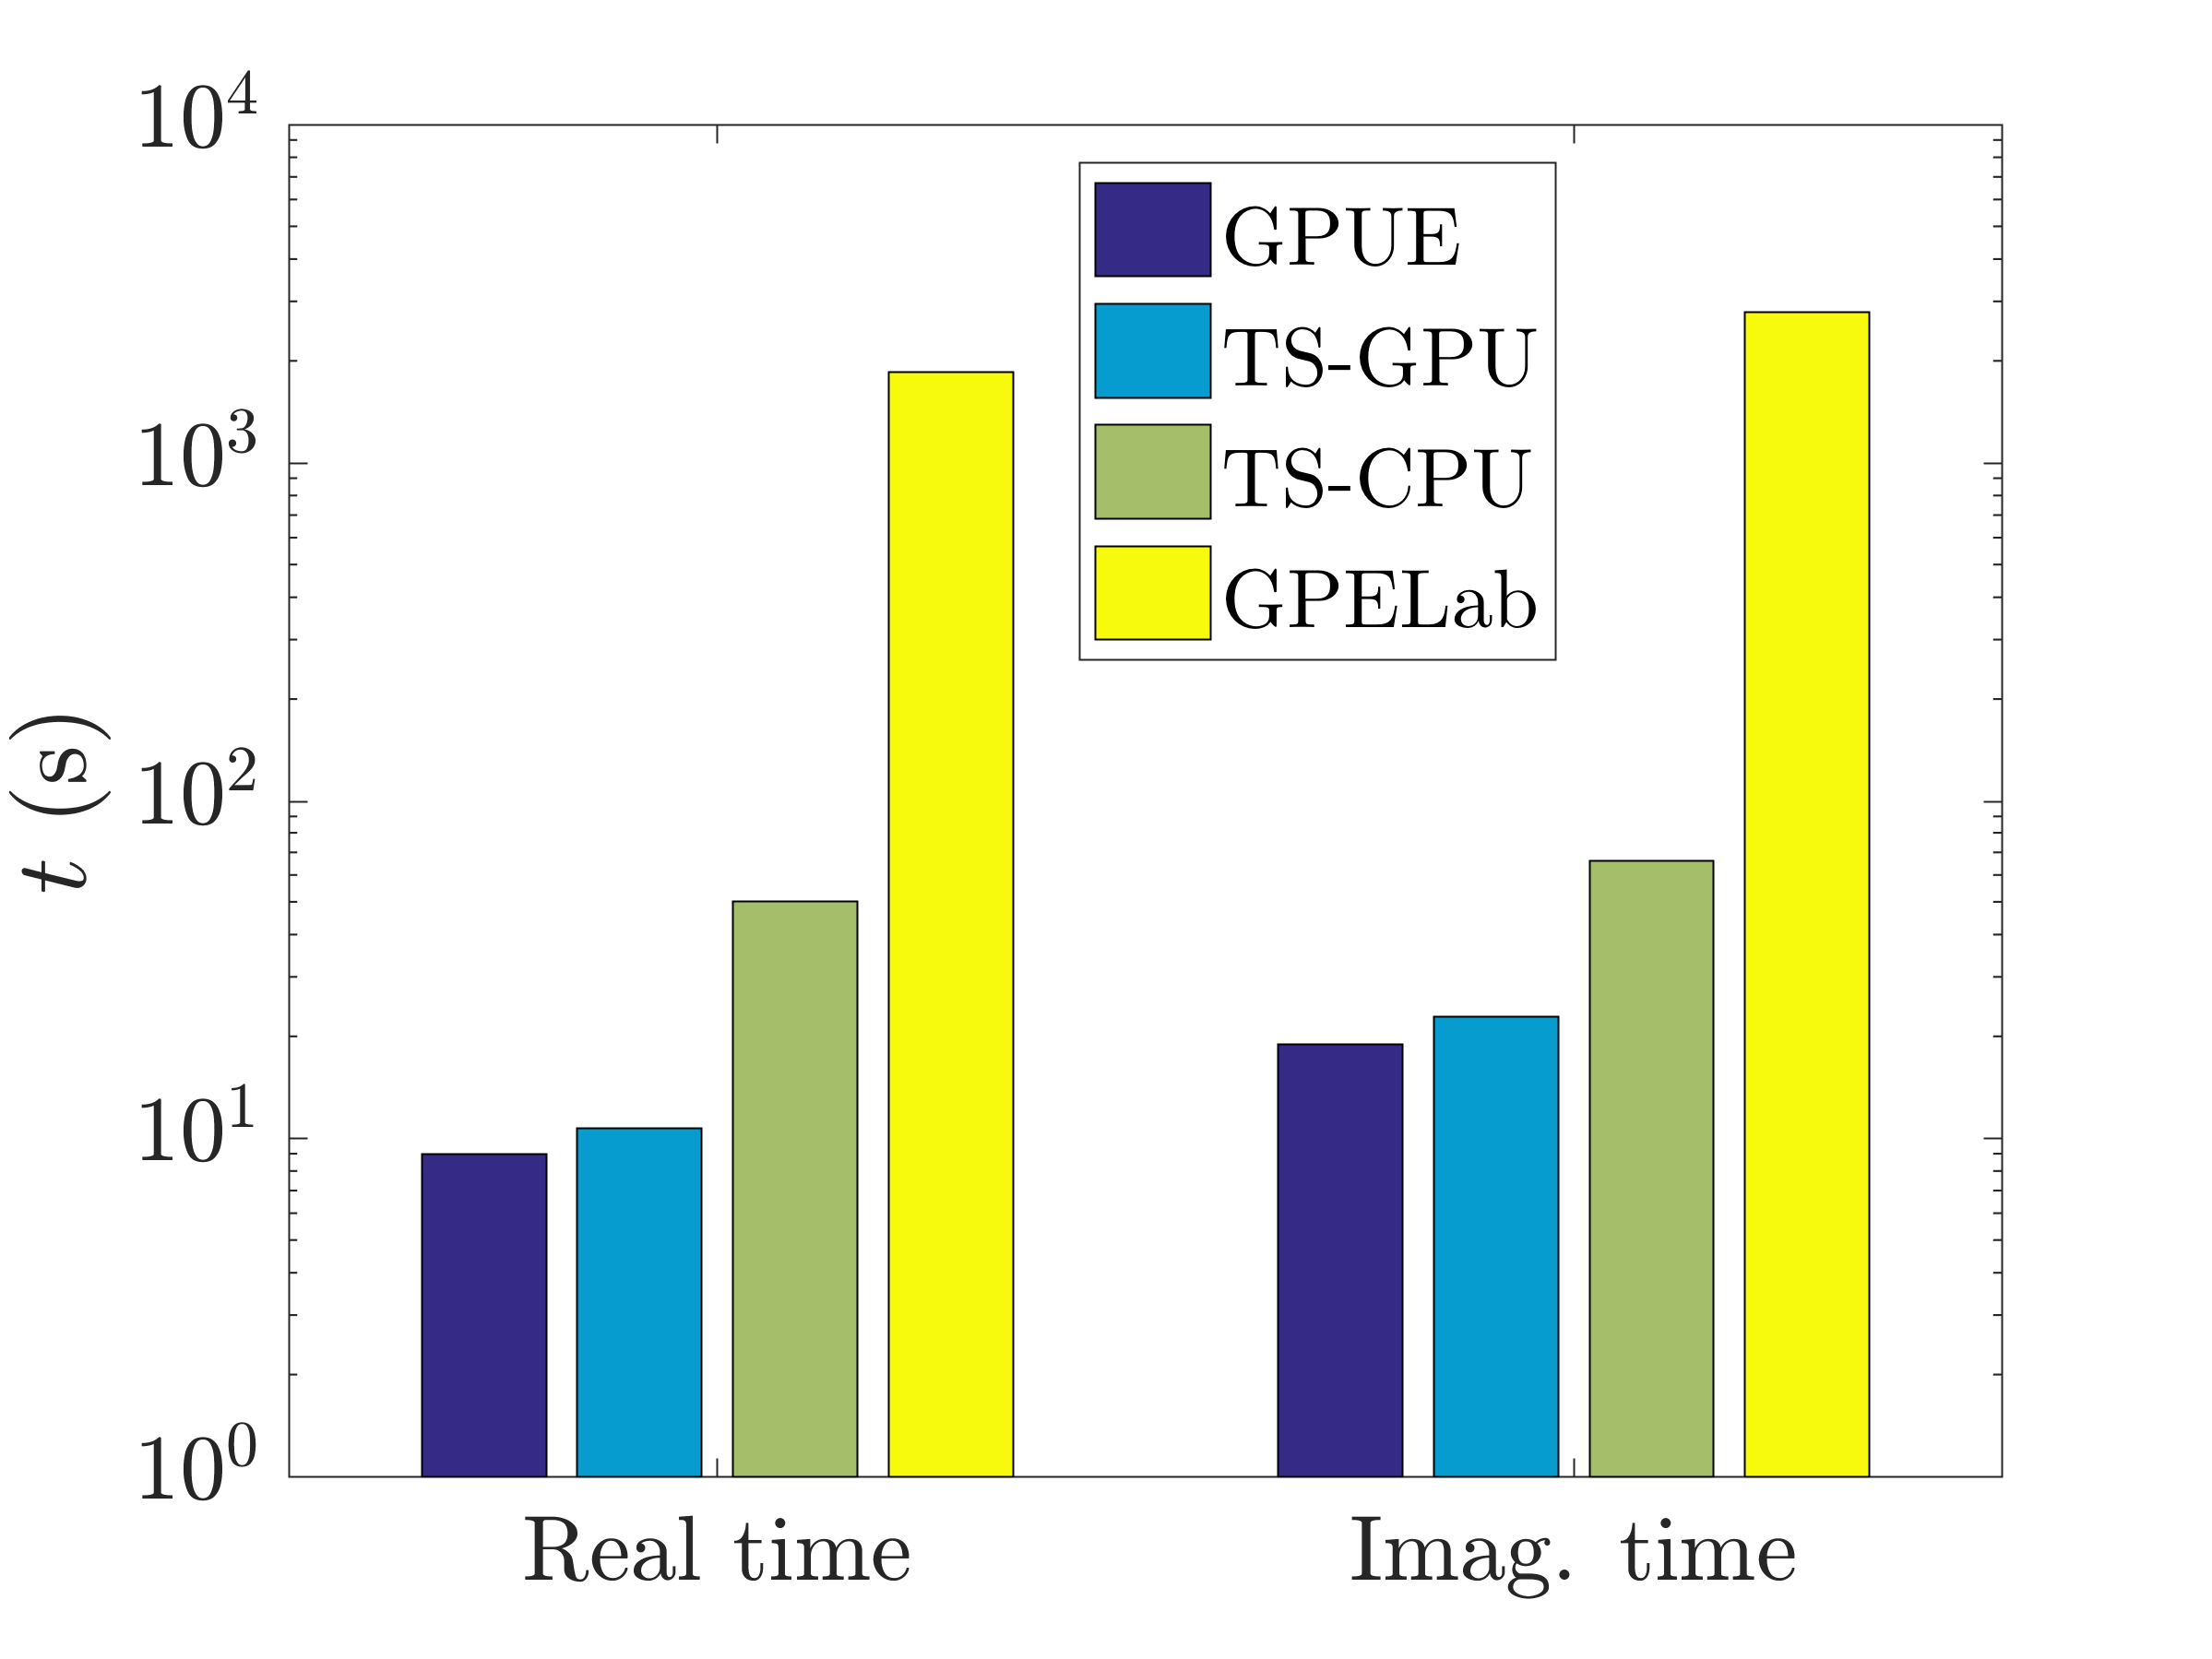
\includegraphics[width=0.5\textwidth,]{ch3_numerics/GPUEvsTS.png}
    \caption{Performance benchmark of GPUE and other simulation packages for the evolution of a harmonically trapped atom in a superposition state between ground and first excited states. Lower numbers are better and give results in faster times. Data adapted from \cite{Wittek:2016}. }
    \label{fig:gpuevsts}
\end{figure}

Figures ~\ref{fig:profile_ev} and \ref{fig:profile_im} demonstrate some of the resulting calls to different segments of the code, with timings given in Tables \ref{tbl:gpue_ev} and \ref{tbl:gpue_im}. The important data of the figures is both the kernel percentage utilisation, and that the operations are mostly saturating the available number of GPU cores. The data shows the average time spent in each individual kernel during both real and imaginary time evolution for 1010 steps at $2^{10}\times 2^{10}$ resolution with (real) and without (imaginary) angular momentum operators. As can be seen, the inclusion of angular momentum operators lead to a performance hit, compared with an imaginary time evolution for a static condensate. While further optimisations can almost always be provided for such simulations, the performance of the software as a whole is defined by its slowest component. In this case the routines are equally met in performance by the Fourier transforms, which are already fully optimised as an external library. As such, improving performance much beyond this with the other kernels will be wasteful in time and resources.

%\iffalse
\begin{figure}
    \centering
    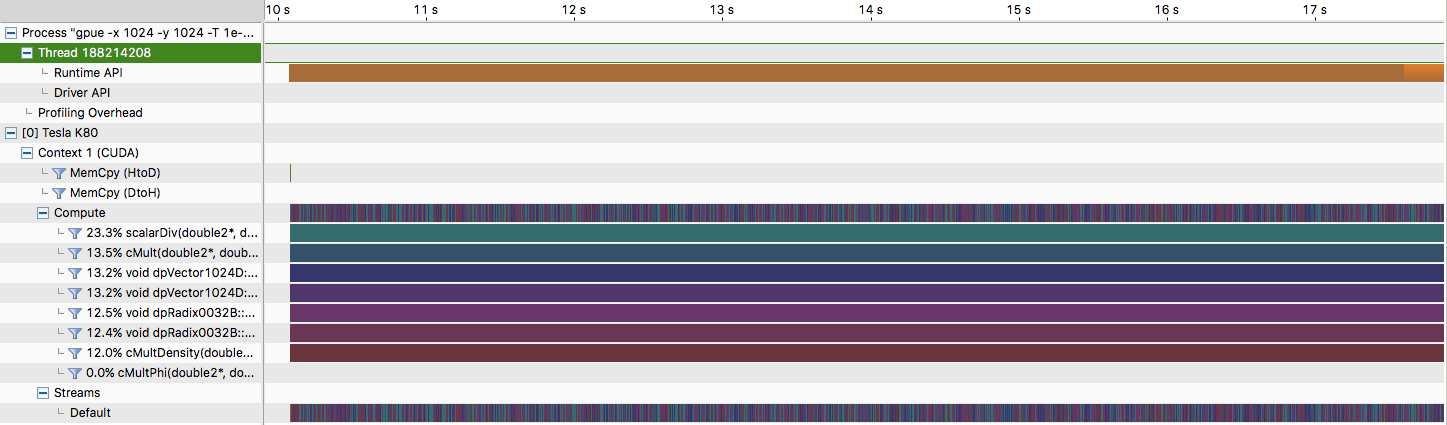
\includegraphics[width=0.98\textwidth,]{ch3_numerics/CUDA/Profiler_ev_1k_1024.png}
    \caption{Nvidia Nsight performance analysis of GPUE for real time evolution simulation for 1010 steps at $2^{10}\times 2^{10}$ resolution. The respective kernel calls and total utilisation are listed on the left.}
    \label{fig:profile_ev}
\end{figure}

\begin{table}
    \scriptsize
    \centering
\begin{tabular}{c|c|c|c|c}
\textbf{Kernel}  & \textbf{Info} & \textbf{Avg. runtime} & \textbf{\# Runs} & \textbf{Total time} \\
\hline
Mem. copy [H2D] & Memory copy from host to GPU & $2.312$ ms & 11 & $25.432$ ms\\
Mem. copy [D2H] & Memory copy from GPU to host & $2.18$ ms & 9 & $19.62$ ms\\
cMult & Complex mult. in time ev. & $0.342$ ms & 3030 & $1.0363$ s\\
cMultDensity & Complex mult. in time ev. for nonlinear op. & $0.456$ ms & 2020 & $0.921$ s \\
scalarDiv & Renorm. of $\Psi$ following FFT & $0.2216$ ms & 8080 & $1.791$ s\\
dpRadix0032B & Internal CUFFT operation & $0.237$ ms & 8080 & $1.915$ s\\
dpVector1024D & Internal CUFFT operation & $0.252$ ms & 8080 & $2.0362$ s\\
\end{tabular}
\caption{Kernel usage and timings for 1010 steps of real time evolution with angular momentum.}\label{tbl:gpue_ev}
\end{table}

\begin{figure}
    \centering
    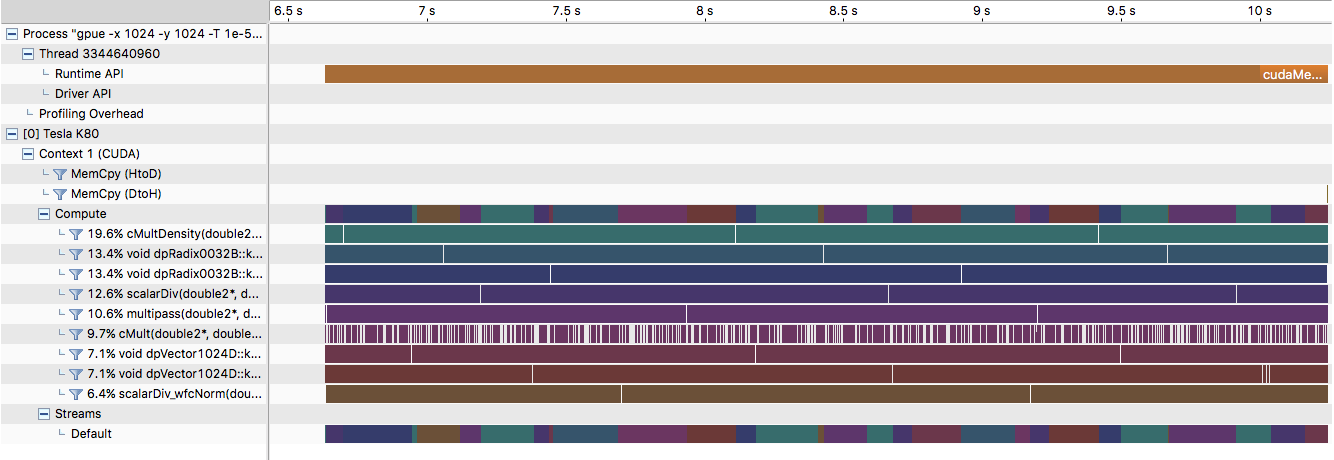
\includegraphics[width=0.98\textwidth,]{ch3_numerics/CUDA/Profiler_im_1k_1024.png}
    \caption{Nvidia Nsight performance analysis of GPUE for imaginary time simulation for 1010 steps at $2^{10}\times 2^{10}$ resolution with angular momentum. The respective kernel calls and total utilisation are listed on the left.}
    \label{fig:profile_im}
\end{figure}

\begin{table}
    \scriptsize
    \centering
\begin{tabular}{c|c|c|c|c}
\textbf{Kernel}  & \textbf{Info} & \textbf{Avg. runtime} & \textbf{\# Runs} & \textbf{Total time} \\
\hline
Mem. copy [H2D] & Memory copy from host to GPU & $2.311$ ms & 3 & $6.933$ ms\\
Mem. copy [D2H] & Memory copy from GPU to host & $1.85$ ms & 5 & $9.25$ ms\\
cMult & Complex mult. in time ev. & $0.342$ ms & 1010 & $0.345$ s\\
cMultDensity & Complex mult. in time ev. for nonlinear op. & $0.346$ ms & 2020 & $0.698$ s \\
multipass & Optimised parallel summation & $0.125$ ms & 3030 & $0.378$ s \\
scalarDiv & Renorm. of $\Psi$ following FFT & $0.221$ ms & 2020 & $0.446$ s \\
scalarDiv_wfcNorm & Normalisation of wavefunction during ev. & $0.226$ ms & 1010 & $0.228$ s\\
dpRadix0032B & Internal CUFFT operation & $0.237$ ms & 4040 & $0.957$ s \\
dpVector1024D & Internal CUFFT operation & $0.251$ ms & 2020 & $0.507$ s \\
\end{tabular}
\caption{Kernel usage and timings for 1010 steps of imaginary time evolution for a non-rotating condensate.}\label{tbl:gpue_im}
\end{table}

A simplified sequence and state diagram combination is given in Figs.~\ref{fig:gpue_seq1} and~\ref{fig:gpue_seq2} which describes the operating process for GPUE. A document listing all aspects of component dependencies and intercommunication is available at~\cite{MLXD_GPUE}. For brevity, we will refer the reader to this location for more information.\footnote{The documentation is built using ~\href{http://www.stack.nl/~dimitri/doxygen/}{Doxygen} with the command ``doxygen ./docs/gpue_doxy.conf'', and requires the \textit{dot} package for figure generation. This may change during future releases.}.

\begin{figure}[]
    \centering
        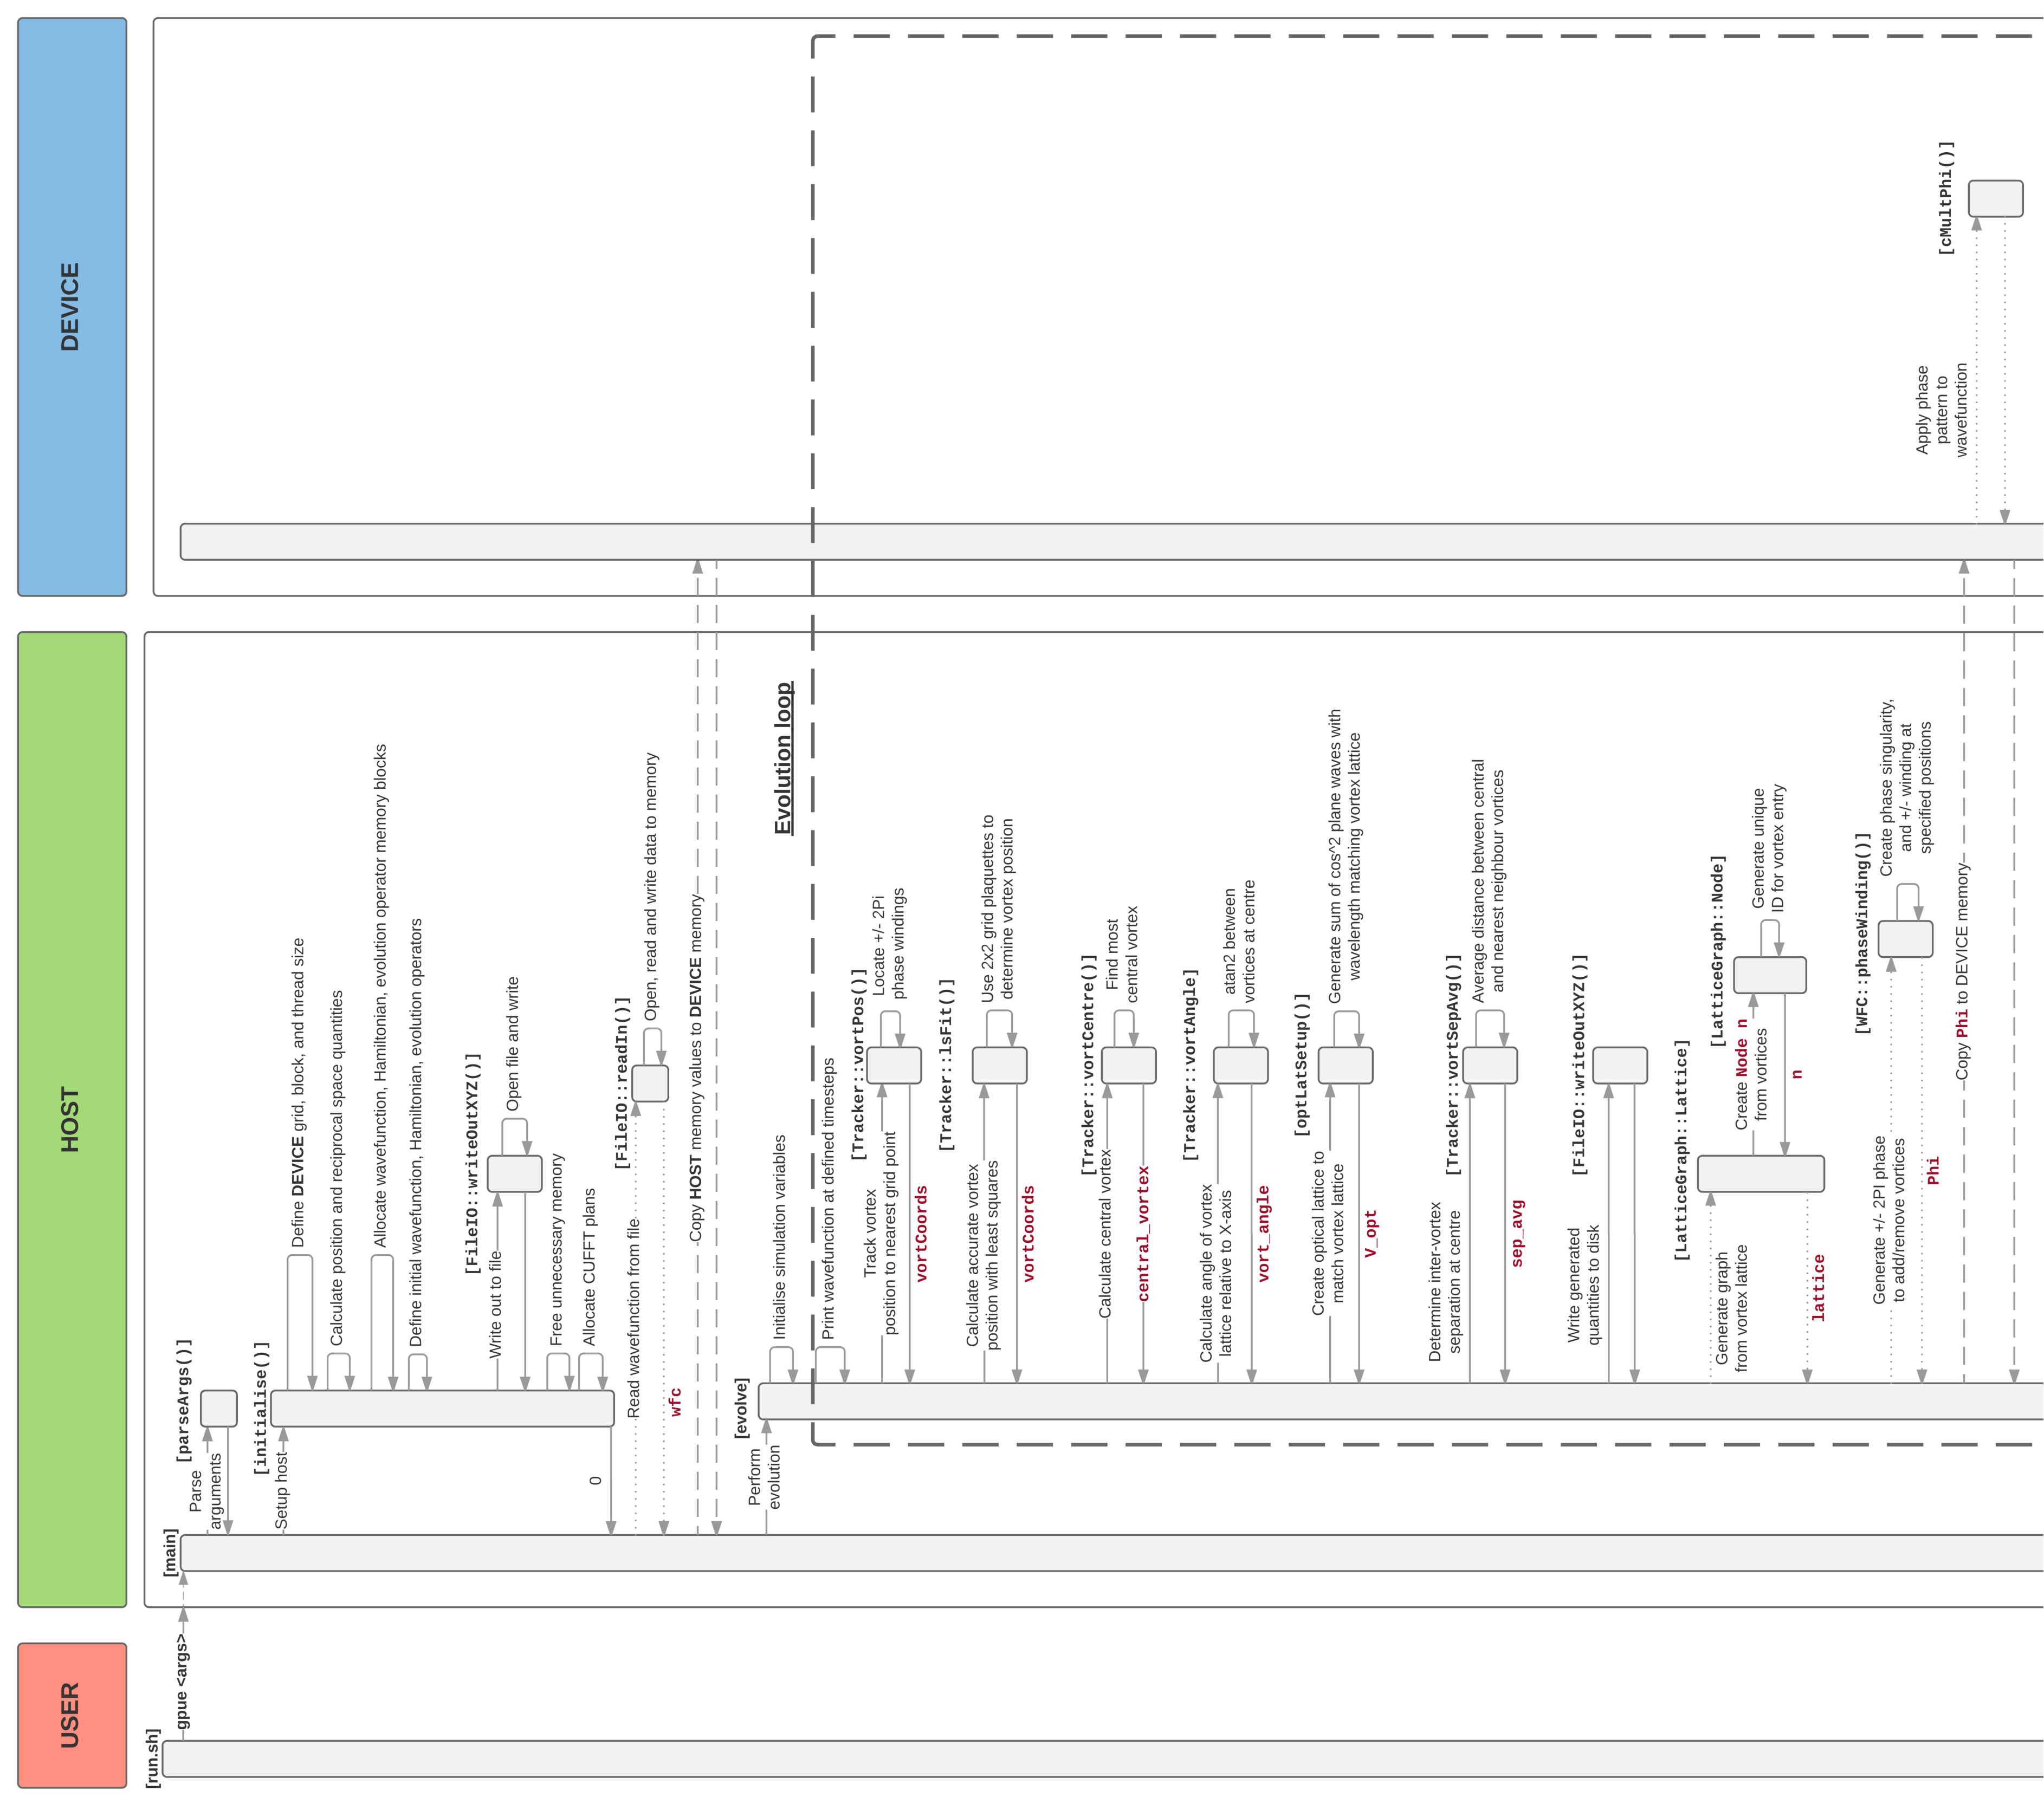
\includegraphics[height=\textwidth,angle=270]{ch3_numerics/GPUE_Seq1}
    \caption{Simplified combined sequence and state diagram for GPUE operation (1 of 2). The operation procedure of GPUE is outlined in sequence from top-to-bottom. While much of the setup and analysis takes place on the host (CPU), the device (GPU) is used to offload all the time-evolution calculations. After setup, the wavefunction and all required operators are sent to the GPU.}
    \label{fig:gpue_seq1}
\end{figure}
\begin{figure}[]
    \centering
        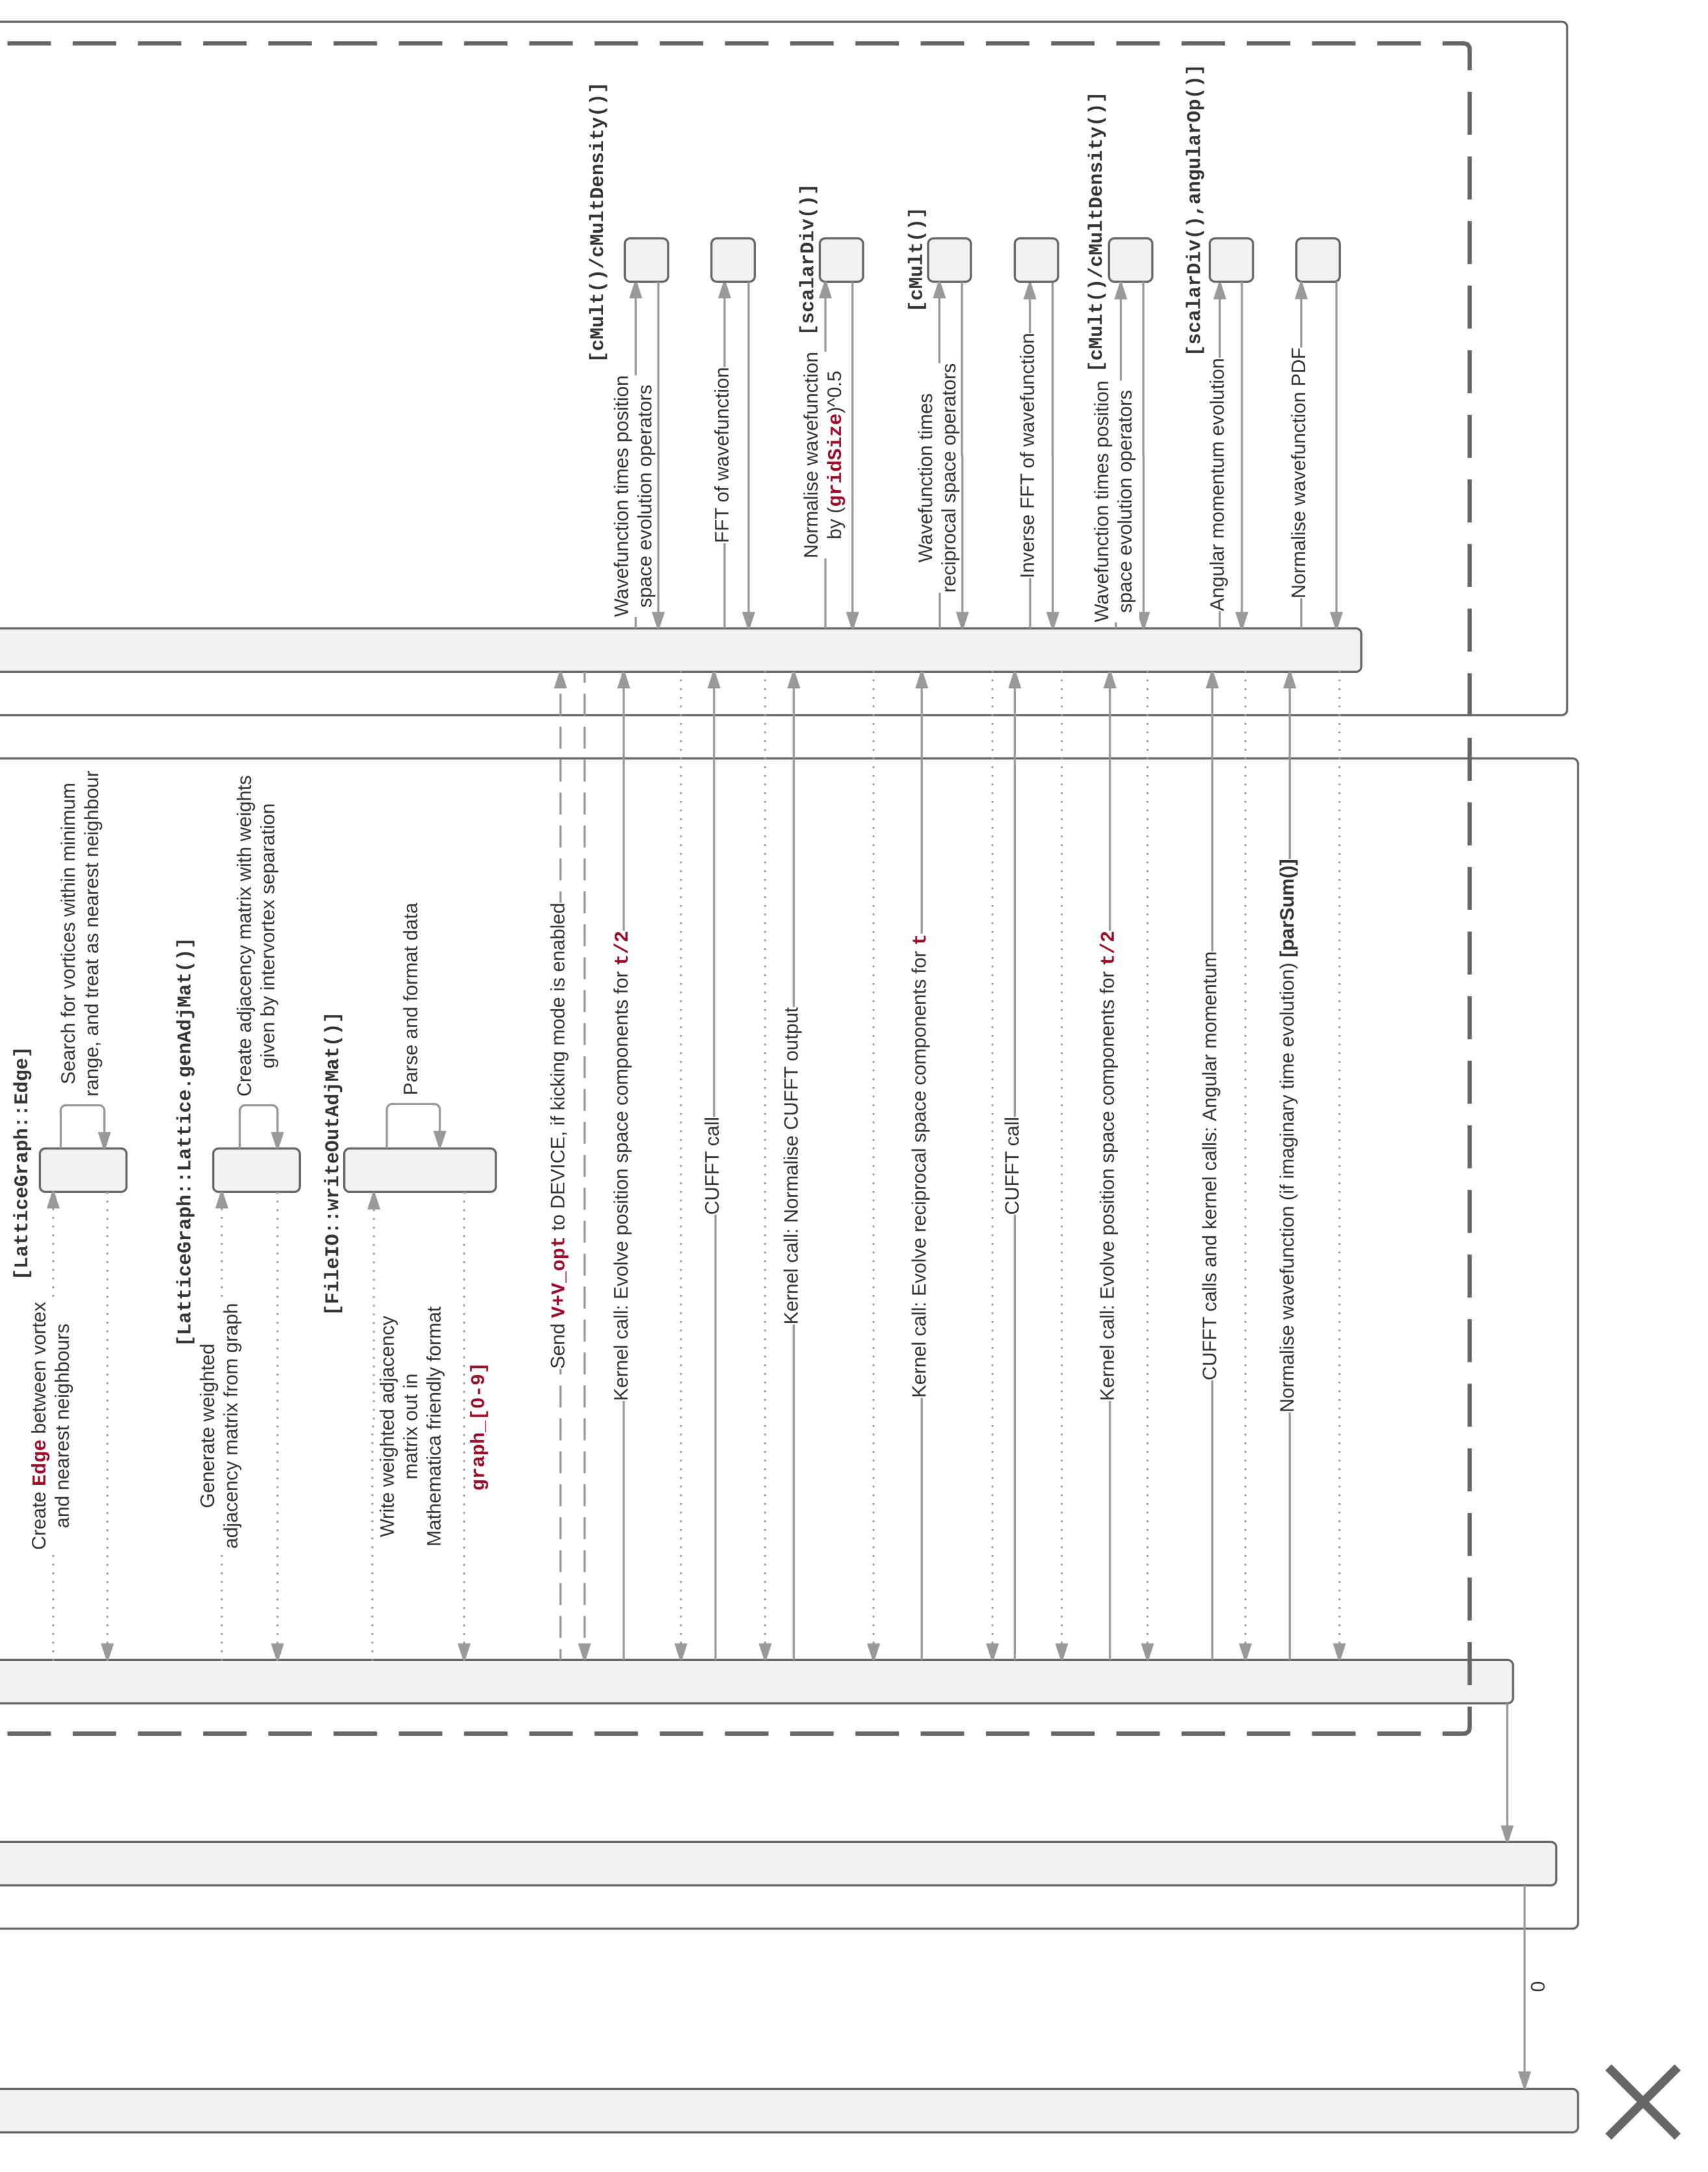
\includegraphics[height=\textwidth,angle=270]{ch3_numerics/GPUE_Seq2}
    \caption{Simplified combined sequence and state diagram for GPUE operation (2 of 2). Following the completion of the time evolution after a predetermined number of steps, the wavefunction is unloaded from the GPU and returned to the CPU for output. Minimising this transfer allows for optimal performance from the device. Further details of dependencies and data flow are given by \cite[docs/gpue.pdf]{MLXD_GPUE}.}
    \label{fig:gpue_seq2}
\end{figure}

\subsection{Angular momentum operators using Fourier split-operator  method}\label{ss:ang_mom_fso}
As discussed earlier, in the presence of large values of angular momentum, the condensate wavefunction will accommodate many vortices. To ensure a well ordered lattice, more consideration is required than to just directly numerically solve the GPE at the required rotation rate. Assuming an initial Gaussian guess, and using the imaginary time evolution algorithm to find the ground state, a large number of vortices will enter the condensate from the edge and compete for lattice sites to form the expected Abrikosov pattern. Due to the highly dense spectrum of the condensate close to the ground state in this regime, only minimal energy shifts will be given for deviations from the perfect Abriksov geometry. As a result, it can take a significantly long time to reach an ordered state for rotation frequencies close to the transverse trapping frequency \cite{Vtx:Mueller_prl_2002}. To overcome this issue, one can choose to follow the ground state of the condensate with a ramp of the rotation rate. This essentially mimics adiabatic evolution, and allows for the determination of the vortex lattice ground state for all rotation frequencies.

The Fourier split-operator algorithm described earlier works well in handling cases where the individual operators live in position or momentum space respectively. However, the angular momentum operators are a combination of both spaces. Taking the angular momentum operator along the $z$-axis, $L_z = xp_y - yp_x$, and applying it to the wavefunction requires each basis element to be in a different space in the different directions. For applying this operator we must therefore Fourier transform along a single dimension, multiply by the respective $\mathbf{k}$-space component, take the inverse, multiply by the respective $\mathbf{r}$-space component in the other direction, and then perform this operation along the other dimensions, summing the results.

This accrues an error which is not encountered using methods that are solely in position or momentum space. Following the process given in Sec.~\ref{sec:fso} the error can be determined by checking the commutativity of the respective components of the angular momentum operator as

 \begin{align}
 	\alpha_1 = [x p_y,-y p_x] &= [x p_y,-y] p_x  -  y[x p_y,p_x] = -[-y,x p_y] p_x + y [p_x, x p_y] \nonumber \\
 		&= -\left( {\cancelto{0}{[-y,x]}} p_y + x [-y,p_y] \right) p_x + y \left( [p_x,x] p_y + x {\cancelto{0}{[p_x,p_y]}} \right) \nonumber \\
 		&= -x {\cancelto{\textrm{i}\hbar}{[-y, p_y]}} p_x + y {\cancelto{-\textrm{i}\hbar}{[p_x,x]}} p_y \nonumber \\
        &= \textrm{i}\hbar \left(x p_x - y p_y \right).
 \end{align}

 The complex error term can be seen as, in the case of the above implemented evolution, allowing the angular momentum operator to change from imaginary time to real-time, and vice-versa in each respective case. To overcome this, we simply swap the application order of the operator components, between odd and even steps during the evolution. Starting with the alternate order we obtain a value of $\alpha_2 = [-y p_x, x p_y] = \textrm{i}\hbar \left(-x p_x + y p_y \right)$. Since we are applying these operators to the condensate we can overcome the error of one term by the application of the other, as
 \begin{equation}
 \exp{\textrm{i} \alpha_1}\exp{\textrm{i} \alpha_2} = 1.
 \end{equation}

 Although alternating will provide a cancellation of this error, it can be assumed that for large timesteps the error will have a significant contribution to the overall dynamics, as the wavefunction evolves during each timestep. For greater accuracy of this method one can perform a decomposition following Eq.~\eqref{eqn:3} for a third-order error, or using the above splitting for second-order.

An example of the density of the ground state and the associated wavefunction phase at a rotation frequency of $\Omega = 0.995\omega_x$ is given in Fig.~\ref{fig:showingoff} at a resolution of $2^{11}\times 2^{11}$ ($2048\times 2048$). Although aliasing may be apparent in the phase, this is due to the limited resolution of the computer monitor (printer). The presence of a well ordered Abrikosov lattice is clearly visible.

 \begin{figure}
     \centering
     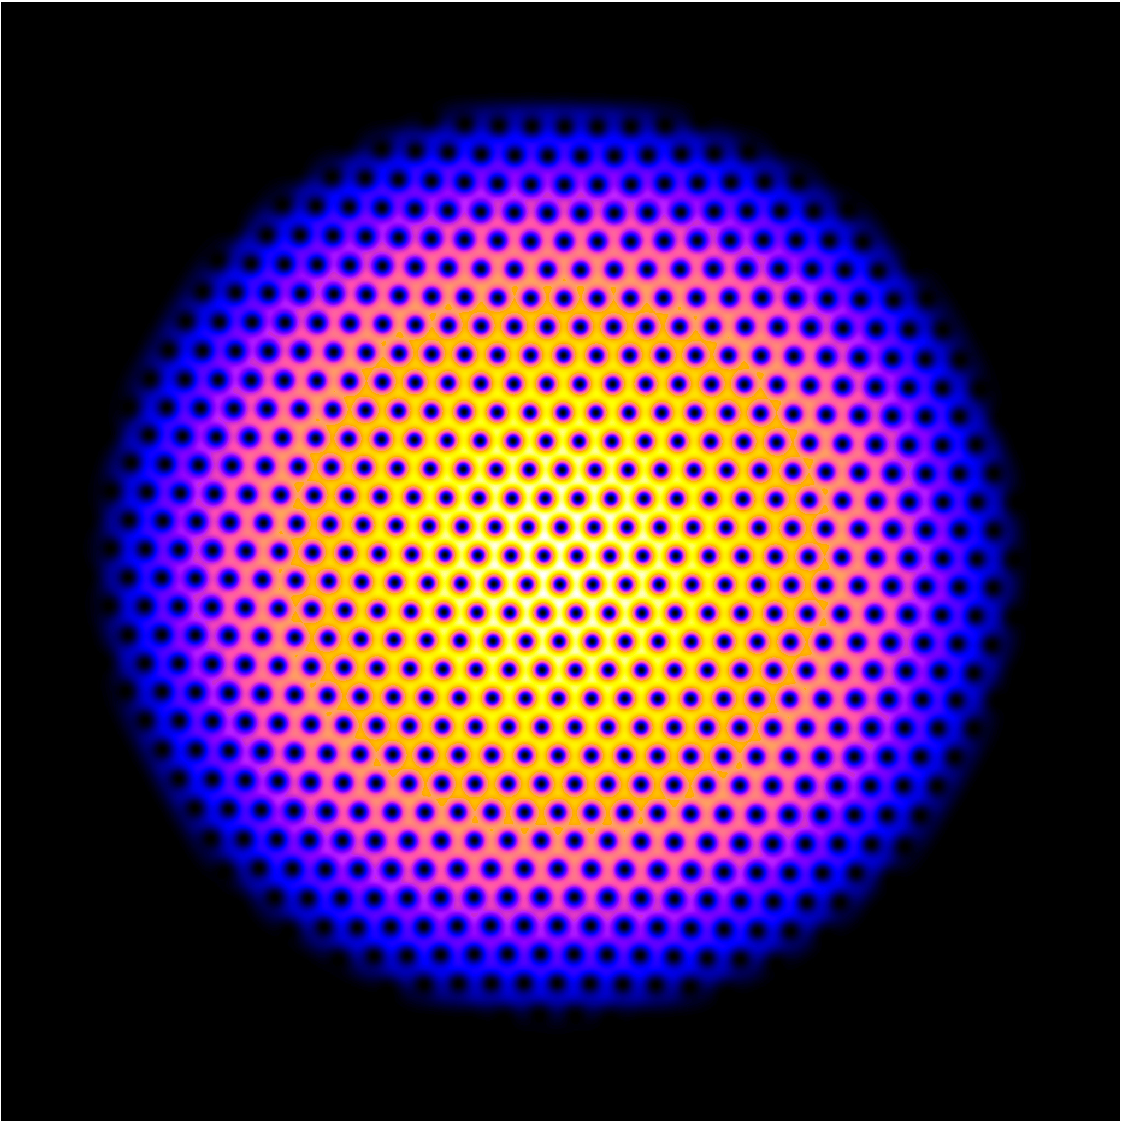
\includegraphics[width=0.45\textwidth,]{ch3_numerics/Rho_995}
     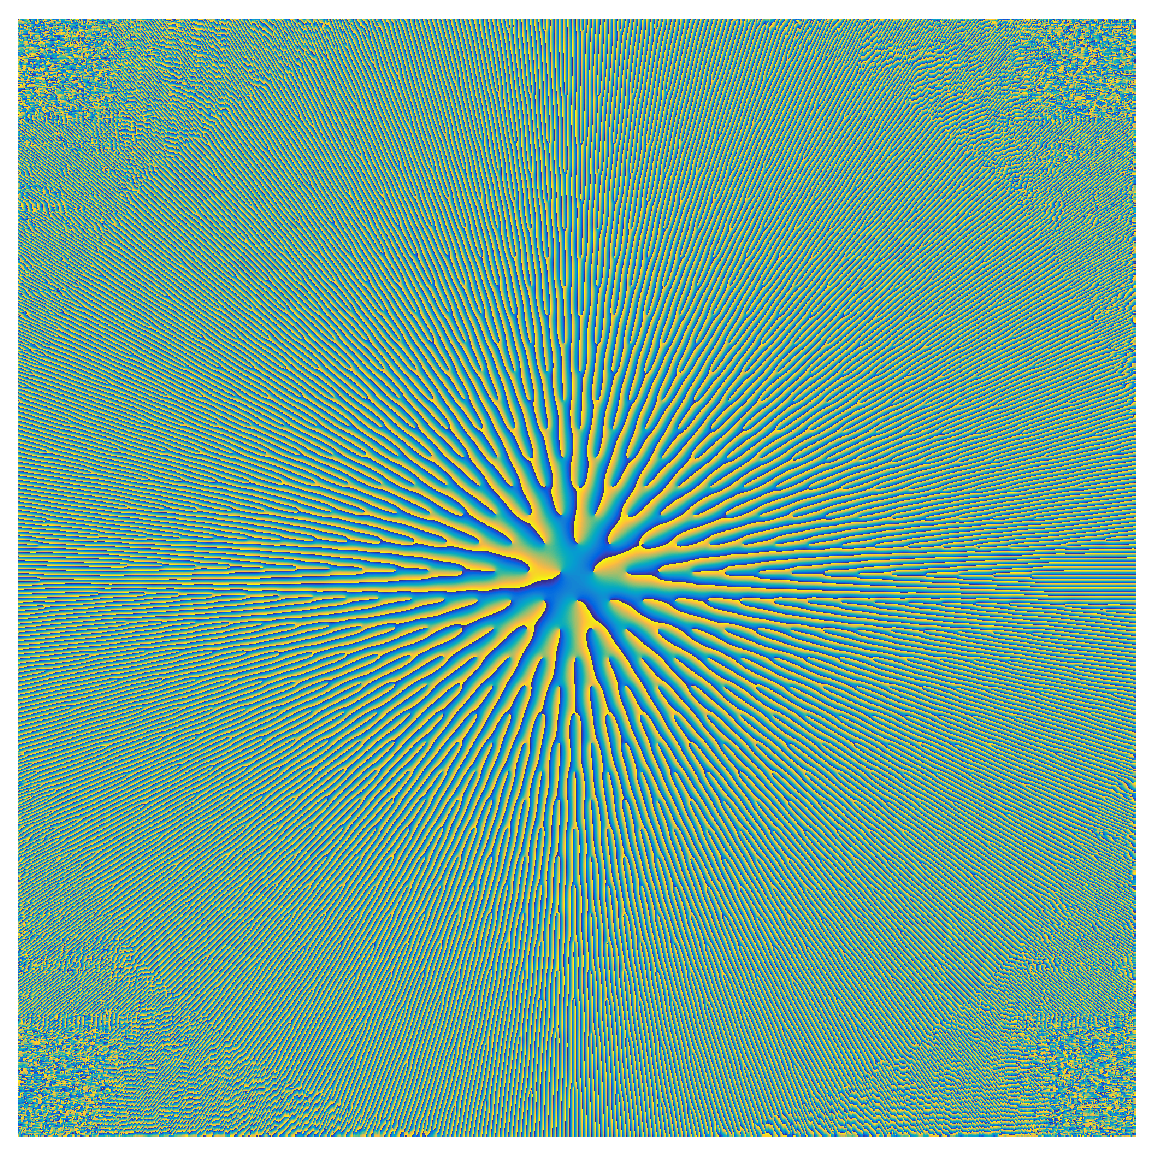
\includegraphics[width=0.45\textwidth,]{ch3_numerics/phi_995}
     \caption{Condensate density (left) and phase (right) at a rotation rate of $\Omega=0.995\omega_x$ for a $2^{11}\times 2^{11}$ grid showing approximately 600 vortices in the visible density regions. For both images the box size is $700~\mu\textrm{m} ~\times ~700~\mu\textrm{m}$.}
     \label{fig:showingoff}
 \end{figure}

 \subsection{Vortex tracking}\label{sec:vortrack}
 To efficiently follow the dynamics of individual vortices, a robust algorithm is needed to track their positions. One could track regions where the density drops to zero. However, this gives very little information on the topological excitation, and may miss many vortices, as the numerical wavefunction may never truly approach this value. A more effective way is to locate the $\pm 2\pi$ charge in the wavefunction phase, which is a signature of quantum vortices. For this we examine each $2\times 2$ subgrid of the underlying lattice and check if the phase rotates from $-\pi$ to $+\pi$ (or vice versa). After an initial pass to identify vortex locations closest the nearest grid element, a least-squares fit is performed to more accurately determine the vortex core position \cite{c42f}. Linear least squares is used generally for an overdetermined linear system $\mathbf{A}\mathbf{r} = \mathbf{b}$, where unique solutions are unlikely to exist. Thus, for a solution, we seek the best fit plane that minimises the error, of the form

 \begin{equation}
 S(\mathbf{r}) = \displaystyle\sum |b_i - \displaystyle\sum A_{ij} r_j |^2
 \end{equation}
 where $S$ is the objective function to be minimised, following $\mathbf{b} = \argmin S(\mathbf{r})$. The solution of this minimisation problem is given by
 \begin{subequations}
\begin{align}
    \mathbf{A} ^{T}\mathbf{A} \mathbf{r} &= \mathbf{A} ^{T}\mathbf{b}, \\
    \mathbf{r} &= (\mathbf{A}^{T}\mathbf{A})^{-1}\mathbf{A}^{T}\mathbf{b}.
\end{align}
\end{subequations}
The best-fit plane is sought of the form
$a_0 c + \displaystyle\sum\limits_{i}^{m} a_i r_i = f(\mathbf{r})$
which for a two-dimensional system, $\mathbf{r} = (x,y)$, is given by the matrix,
\begin{equation}
    \mathbf{A} = \left(
    \begin{array}{ccc}
        0 & 0 & 1 \\
        0 & 1 & 1 \\
        1 & 0 & 1 \\
        1 & 1 & 1
    \end{array}\right).
\end{equation}
The above matrix is composed of all possible planes that can fit over a square $2\times 2$ grid plaquette,
and
\begin{equation}
    \mathbf{b} = \left(
    \begin{array}{cccc}
        \Psi(x_0,y_0) & \Psi(x_0,y_1) & \Psi(x_1,y_0) & \Psi(x_1,y_1)
    \end{array} \right)^{T},
\end{equation}
are the wavefunction values around the sampled $2\times 2$ grid.
Upon evaluating the vector $\mathbf{r}$ above, one can obtain the best fit plane  solution as
\begin{equation}\left(
    \begin{array}{c}
        x \\
        y \\
        c
    \end{array}\right)
    = \left(
    \begin{array}{c}
        {\left( -\Psi(x_0,y_0) + \Psi(x_0,y_1) - \Psi(x_1,y_0) + \Psi(x_1,y_1) \right)}{/2} \\
        {\left( -\Psi(x_0,y_0) - \Psi(x_0,y_1) + \Psi(x_1,y_0) + \Psi(x_1,y_1) \right)}{/2} \\
        3\Psi(x_0,y_0) + \Psi(x_0,y_1) - \Psi(x_1,y_0) - \Psi(x_1,y_1)
    \end{array}\right).
\end{equation}

The goal is to find where both the real and imaginary components cross through zero, and thus we seek a solution of the form $x + y = -c$. Rearranging the above equations as
\begin{equation}\left(
    \begin{array}{cc}
        \Re(x) & \Re(y) \\
        \Im(x) & \Im(y) \\
    \end{array}\right)
    \left(
    \begin{array}{c}
        \delta x \\
        \delta y
    \end{array}\right)
    = -
    \left(
    \begin{array}{c}
        \Re(c) \\
        \Im(c)
    \end{array}\right),
\end{equation}
and again solving the linear system by inverting the left-hand matrix and multiplying across allows one to seek the corrections to the vortex position, $\delta \mathbf{r} = (\delta x, \delta y )$.

 With this, we can accurately determine the position of the vortices with high precision. To track their motion during the evolution, we create an initial list of positions and give each vortex a unique identifier (UID). Assuming the vortex cores can travel a limited distance (some multiple of the grid resolution) between time steps, we can say at subsequent times which vortex has moved to the newly found positions.

 This process is performed by representing the vortices as a graph, each with an assigned unique identifier, associated location, phase winding and on/off flag. Edges are created between vortices that are separated by at most root-two the average of the inter-vortex spacings. A finite boundary is chosen to examine only vortices in areas of significant condensate density, since vortices can easily appear and disappear close to the condensate boundary. Any vortex which appears without association to an initial vortex, or any tracked vortex that crosses the boundary, is switched off and remains so for all analysis. A graph for an initial ($t=0$) vortex lattice shown in Fig.~\ref{fig:graphit}, with the identifiers indicated on each node, and the neighbouring distances indicated by the edge weights. %The almost perfect triangular structure is clearly confirmed. %%This is a graph, not a location plot. Positions are chosen at mathematicas discretion

 \begin{figure}
     \centering
     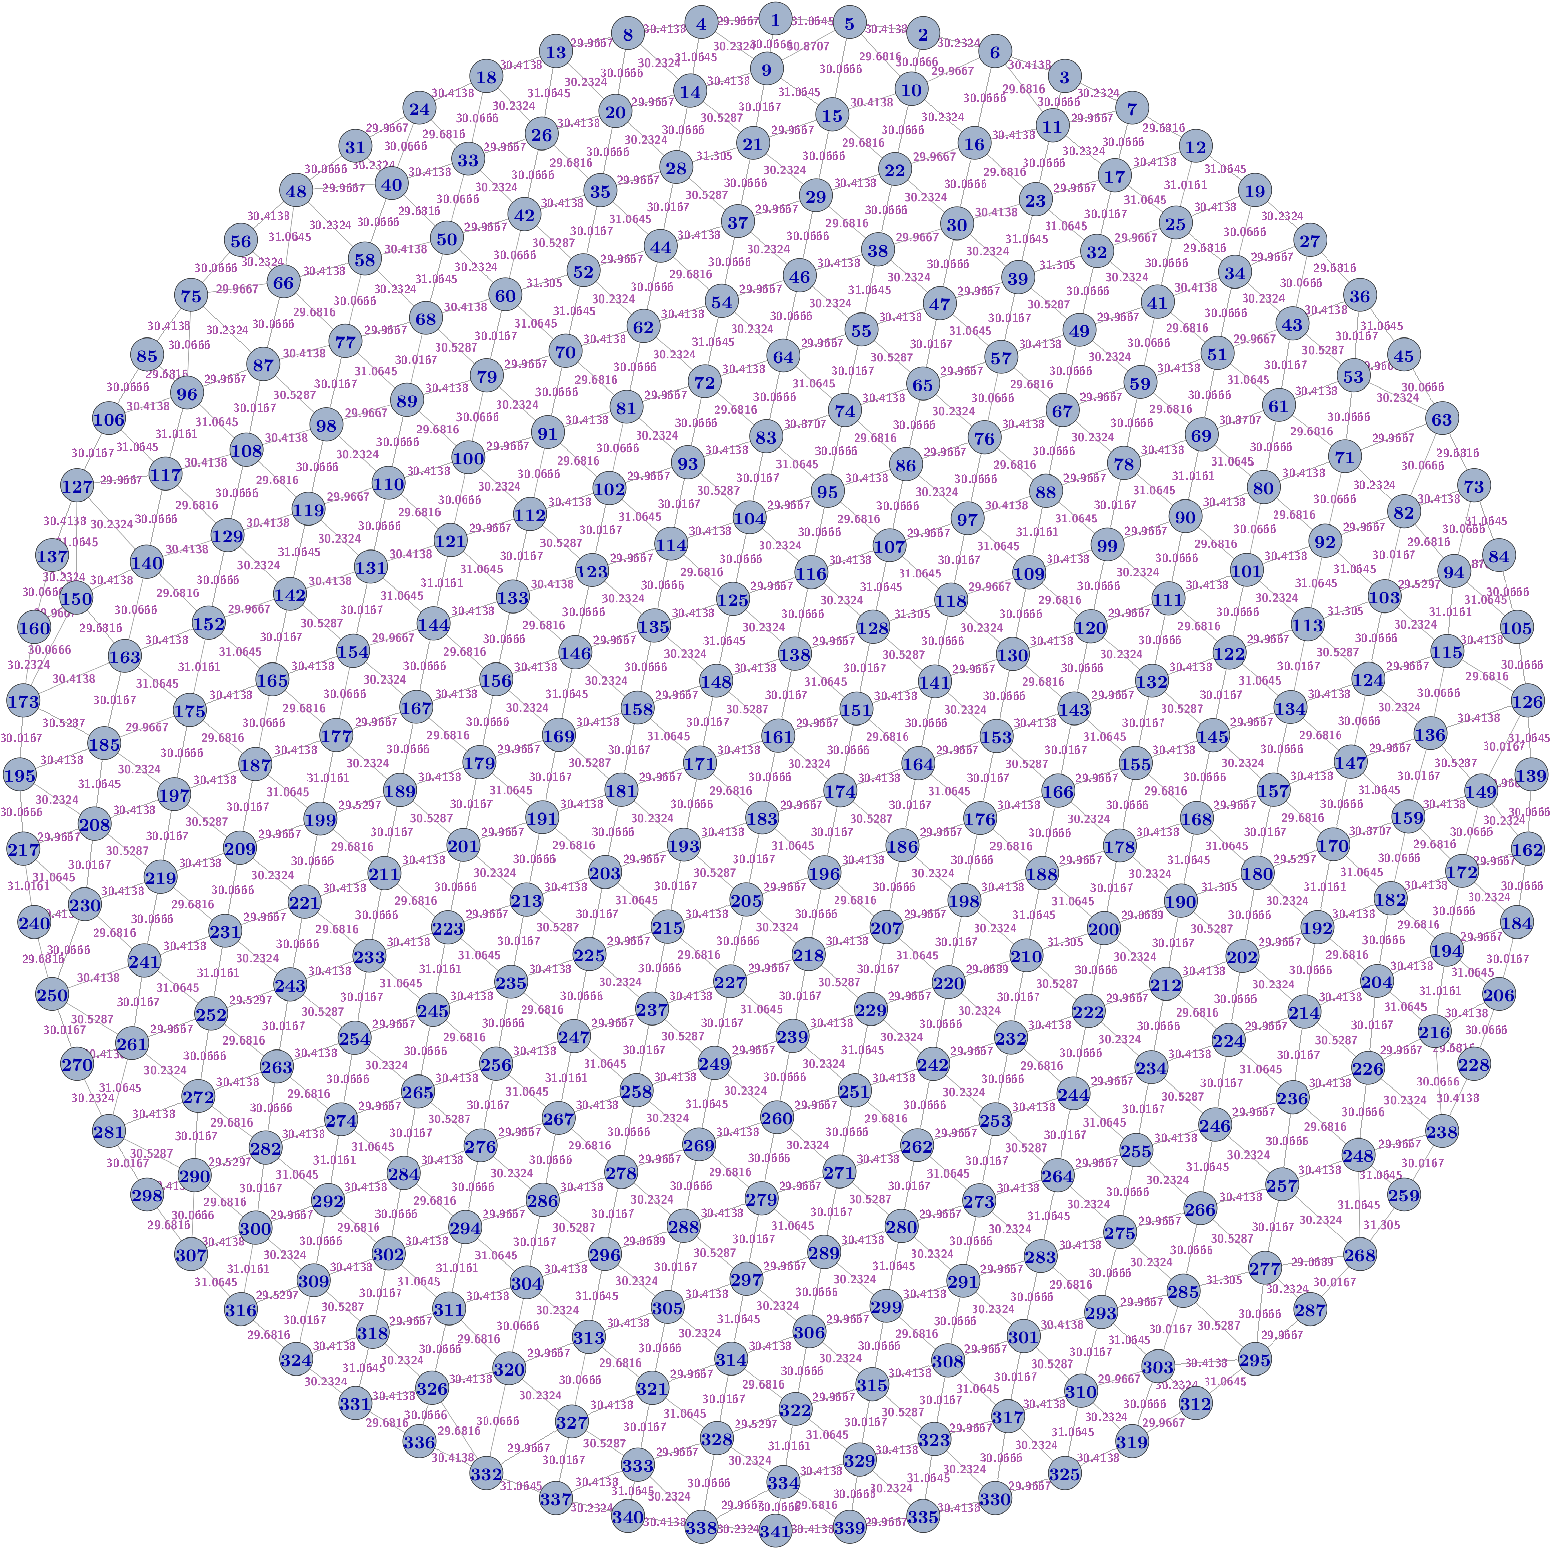
\includegraphics[width=0.98\textwidth,]{ch3_numerics/Graph_full}
     \caption{Graph of vortex lattice positions indicating the vortex identifier and the intervortex distances in units of grid-spacing $\Delta= \Delta x = \Delta y$. A hard-walled boundary is chosen such that the vortex distances remain almost uniform, and are shown here with a mean value of $\bar{r} = 30.2451$ and variance of $\sigma^2 = 0.16118$.}
     \label{fig:graphit}
 \end{figure}
